\documentclass[12pt, bachelor, substylefile = algo_title.rtx]{disser}

\usepackage[a4paper,
            left=1.5cm, right=1.5cm,
            top=2cm, bottom=2cm,
	 headsep=1cm, footskip=1cm]{geometry}
\usepackage[T2A]{fontenc}
\usepackage[utf8]{inputenc}
\usepackage[english]{babel}
\usepackage{amsmath, amsthm}
\usepackage{hyperref}
\usepackage{amsfonts}
%\usepackage{indentfirst}
\usepackage{xcite}
\usepackage{xr}
\usepackage{outlines}
\usepackage{mathtools}
\usepackage{subcaption}
%\usepackage{newtxtext,newtxmath}
\usepackage[final]{pdfpages}


\DeclarePairedDelimiter\ceil{\lceil}{\rceil}
\DeclarePairedDelimiter\floor{\lfloor}{\rfloor}
\newcommand{\Hyp}{\ensuremath{\mathbb{H}}}
\newcommand{\Pb}{\mathcal{P}}
\newcommand{\ME}{\mathbb{E}}
\newcommand{\med}{\mathbb{M}}
\newcommand{\Proba}{\mathbb{P}}
\newcommand{\VAR}{\mathbb{D}}
\newcommand{\varD}{\mathbf{D}}
\newcommand{\eps}{\varepsilon}
\newcommand{\varZ}{\mathbf{Z}}
\newcommand{\varV}{\mathbf{V}}
\newcommand{\varW}{\mathbf{W}}
\newcommand{\varY}{\mathbf{Y}}
\newcommand{\varX}{\mathbf{X}}
\newcommand{\varR}{\mathbf{R}}
\newcommand{\varS}{\mathbf{S}}
\newcommand{\varU}{\mathbf{U}}
\newcommand{\ind}{\mathbb{I}}
\newcommand{\Real}{\mathbb{R}}
\newcommand{\Sample}{\varV_1,\varV_2,\dots,\varV_m}
\newcommand{\Samplex}{\varX_1,\varX_2,\dots,\varX_n}
\DeclareMathOperator{\sign}{sign}

\newcommand{\specialcell}[2][c]{%
  \begin{tabular}[#1]{@{}c@{}}#2\end{tabular}}

\theoremstyle{definition}
\newtheorem{theorem}{Theorem}
\newtheorem{definition}{Definition}
\newtheorem{assumption}{Assumption}
\newtheorem{lemma}{Lemma}
\newtheorem{example}{Example}
\newtheorem{proposition}{Proposition}
\newtheorem{conseq}{Consequence}

\setcounter{tocdepth}{2}


\begin{document}

\institution{FEDERAL STATE AUTONOMOUS EDUCATIONAL INSTITUTION\\
OF HIGHER EDUCATION\\
ITMO UNIVERSITY
}
\title{Report on learning practice \#4}


\topic{\normalfont\scshape %
Stationarity of the processes}
\author{Dmitry Grigorev,\\ Eugenia Khomenko,\\ Efim Podkovirkin,\\ Arina Syrchenko}

\city{St. Petersburg}
\date{2022}

\maketitle

\tableofcontents

\section{Data description}

Let $D$ be the modified dataset on Narvik roads. The features here are:

\begin{outline}
\1lat\_ — latitude
\1 lon\_ — longitude
\1 State\_ — word description of road state (1: 'dry', 2: 'moist', 3: 'wet', 4: 'icy', 5: 'snowy', 6: 'slushy')
\1 Ta\_mean,Ta\_min,Ta\_max — atmosphere temperature
\1 Tsurf\_mean,Tsurf\_min,Tsurf\_max — surface temperature
\1 Water\_mean,Water\_min,Water\_max — water layerw width (0 -- 3 $mm$)
\1 Speed\_mean,Speed\_min,Speed\_max — wind speed (in knots, $5\ knots \approx 9.3\ km/h$)
\1 Height\_mean,Height\_min,Height\_max — height of location above mean sea level
\1 Tdew\_mean,Tdew\_min,Tdew\_max — dew point ($Celsius$)
\1 Friction\_mean,Friction\_min,Friction\_max — friction value ( 0 -- 1, 0 means no friction)
\1 Date,Time, date\_time, FullDate — time and date
\1 Direction\_min,Direction\_max — wind direction ($degrees$)
\1 ClosestCity, location
\1 maxtempC,mintempC — day maximum and minimum of temperature ($Celsius$)
\1 totalSnow\_cm — total snowfall ($cm$)
\1 sunHour — passed sun energy in $Sun-Hours$ (A $Sun-Hour$ is "1000 watts of energy shining on 1 square meter of surface for 1 hour")
\1 uvIndex — ultraviolet index
\1 moon\_illumination — moon phase ($percents$)
\1 moonrise — time of Moon rise
\1 moonset — time of Moon set
\1 sunrise — time of Sun rise
\1 sunset — time of Sun set
\1 DewPointC — hourly dew point measurement ($Celsius$)
\1 FeelsLikeC — hourly Feels-like temperature ($Celsius$)
\1 HeatIndexC — hourly heat index ($Celsius$)
\1 WindChillC — hourly wind-chill index ($Celcius$) 
\1 WindGustKmph — hourly wind gust measure ($km/h$)
\1 cloudcover — hourly cloud cover index ($percents$)
\1 humidity — hourly humidity ($percents$)
\1 precipMM — hourly precipitation ($mm$)
\1 pressure — hourly atmosphere pressure ($mbar$)
\1 tempC — hourly atmosphere temperature ($Celsius$)
\1 visibility — hourly visibility (0--10, 0 means poor visibility)
\1 winddirDegree — hourly wind direction ($degrees$)
\1 windspeedKmph — hourly wind speed ($km/h$)
\end{outline}


\begin{figure}[!h]
\centering
   \begin{minipage}{0.7\textwidth}
     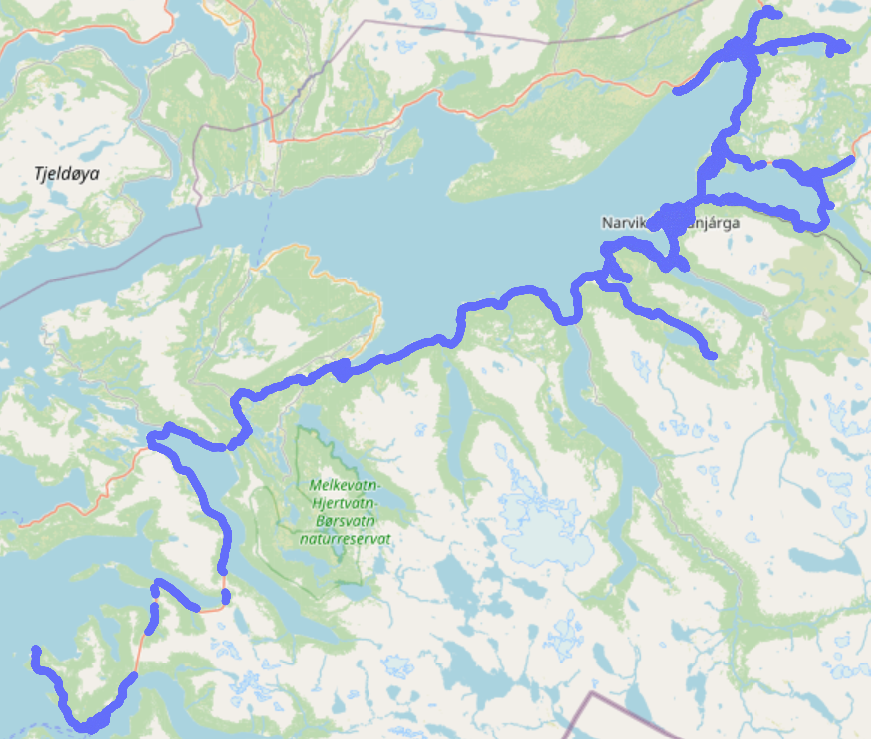
\includegraphics[width=\linewidth]{geography}
   \end{minipage}
\caption{Geography of the data}
\label{fig: }
\end{figure}

\section{Substantiation of chosen sample}
Friction\_mean, Water\_mean and Tsurf\_mean are chosen as targets. As predictors we chose variables Height\_mean and Speed\_mean. The data are collected across the map in fig. \ref{fig: } and they are too inhomogeneous and non-equidistant in time. 

To tackle the latter problem, we did downsample according to the time with the period of $3$ minutes with mean aggregation of the variables. This operation generated some missing data which occurred due to the time intervals between two consequential observation larger than $3$ minutes in time. Firstly, we selected only first 300 observations from the beginning of the measurements to study only the corresponding geographic location (neighborhood of Øyjord town). Secondly, there are a few of missing data which we filled by rolling mean of order 3 since the gaps are small and the close observations are likely to be similar.

\section{Stationary and covariance/correlation function analysis}
At first, we drew the series themselves with the fitted polynomials of the 9th degree which approximate the series' possible trends. They are all shown in figure \ref{fig: 1}.

\begin{figure}[!h]
   \begin{minipage}{.48\textwidth}
     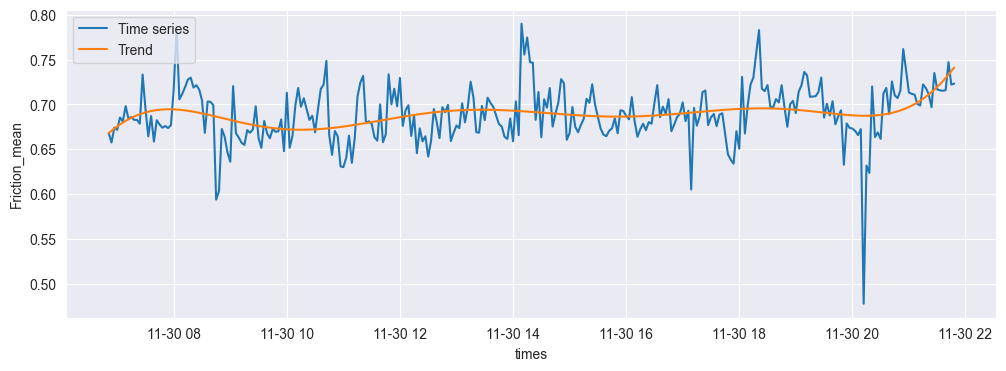
\includegraphics[width=\linewidth]{trend1}
   \end{minipage} \hfill
\begin{minipage}{.48\textwidth}
     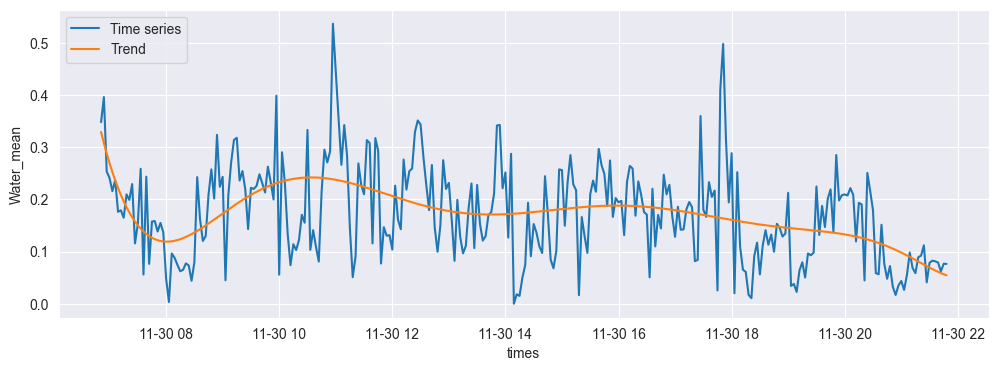
\includegraphics[width=\linewidth]{trend2}
   \end{minipage}\\
\begin{minipage}{.48\textwidth}
     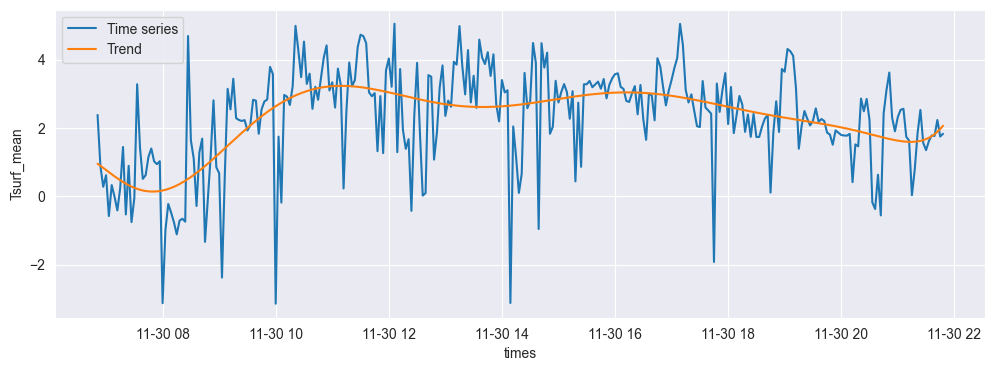
\includegraphics[width=\linewidth]{trend3}
   \end{minipage} \hfill
\begin{minipage}{.48\textwidth}
     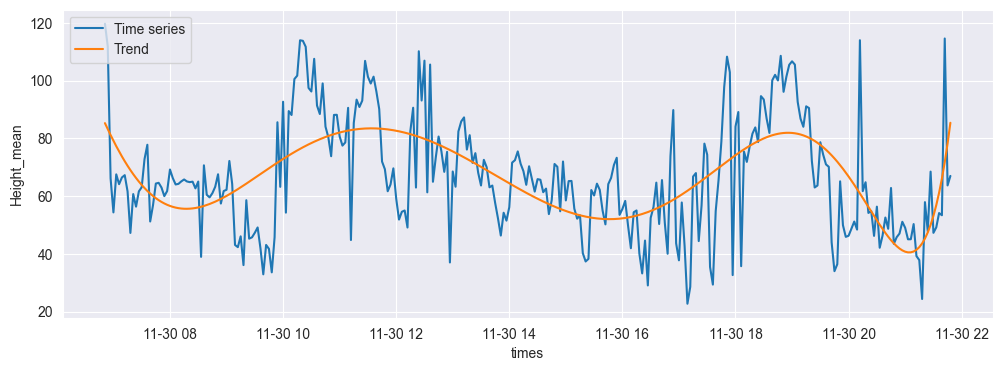
\includegraphics[width=\linewidth]{trend4}
   \end{minipage}\\
\centering
\begin{minipage}{.48\textwidth}
     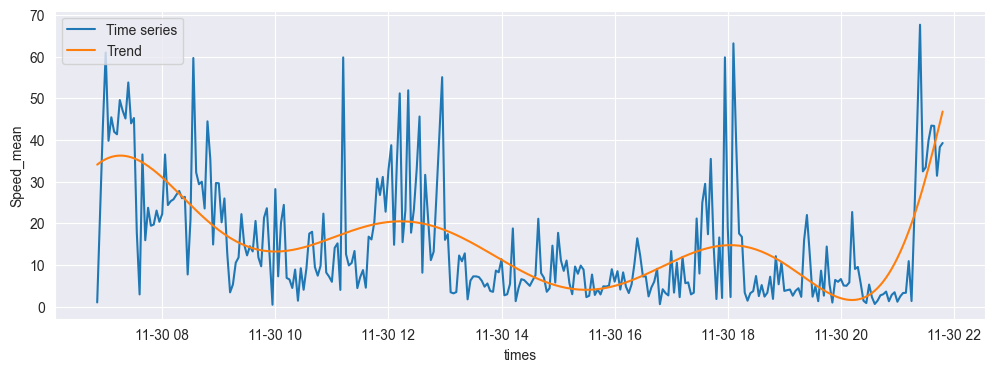
\includegraphics[width=\linewidth]{trend5}
   \end{minipage}
\caption{The histogram of the generated sample vs the mixture's density and the histogram of observed Friction\_mean}
\label{fig: 1}
\end{figure}

Although Friction\_mean serial looks stationary, we intentionally removed both its learnt trend and the trends of other features each of which has a certain tendency. The resulted series are shown in figure \ref{fig: 2} where for each of the variable under the study the estimates of mean and variance functions of the series are provided to infer weak stationarity.

\begin{figure}[!h]
   \begin{minipage}{.48\textwidth}
     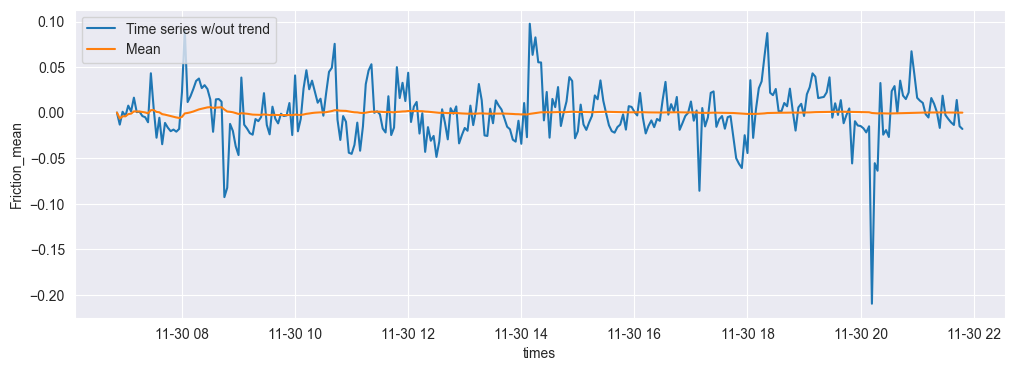
\includegraphics[width=\linewidth]{mean1}
   \end{minipage} \hfill
\begin{minipage}{.48\textwidth}
     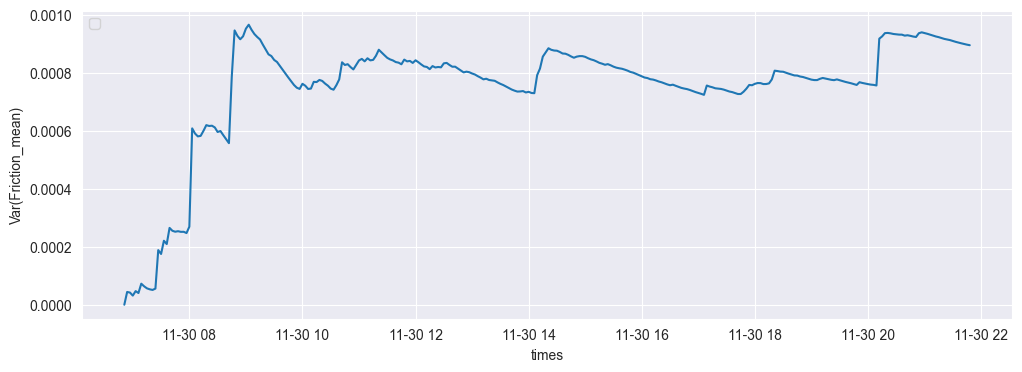
\includegraphics[width=\linewidth]{var1}
   \end{minipage}
   \begin{minipage}{.48\textwidth}
     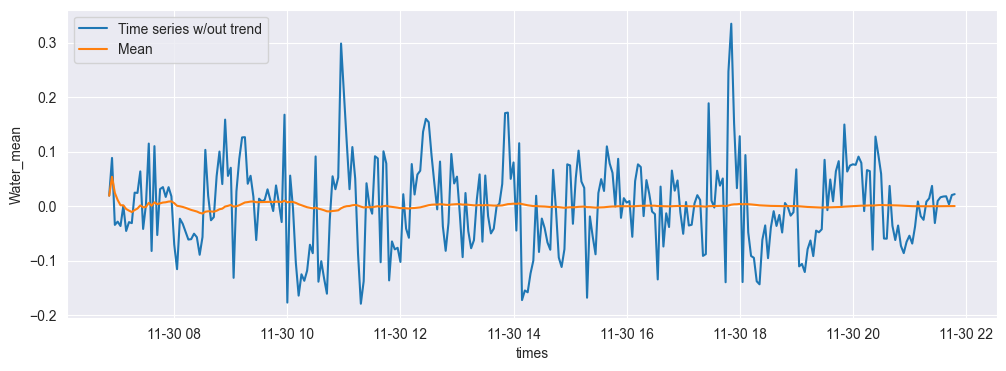
\includegraphics[width=\linewidth]{mean2}
   \end{minipage} \hfill
\begin{minipage}{.48\textwidth}
     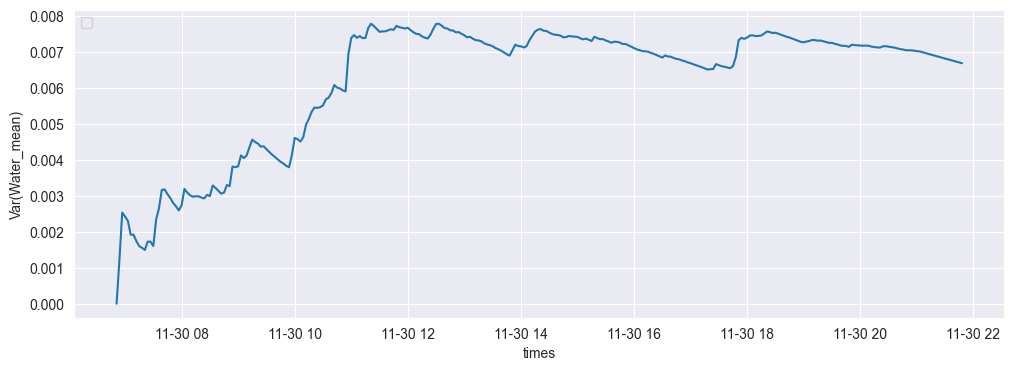
\includegraphics[width=\linewidth]{var2}
   \end{minipage}
   \begin{minipage}{.48\textwidth}
     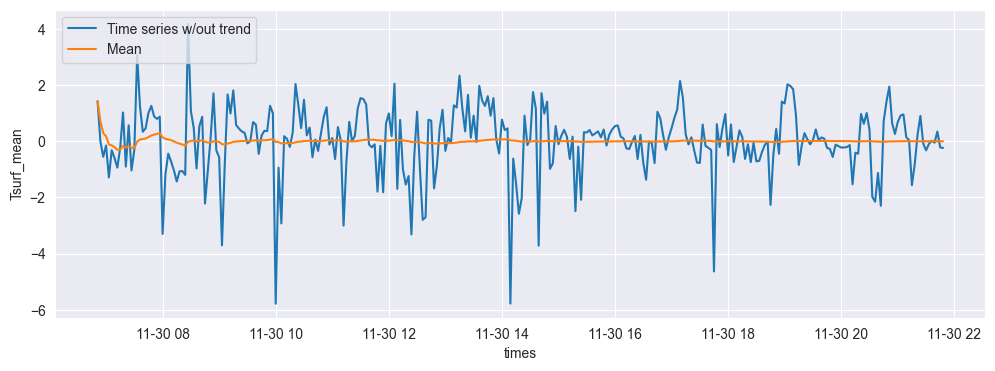
\includegraphics[width=\linewidth]{mean3}
   \end{minipage} \hfill
\begin{minipage}{.48\textwidth}
     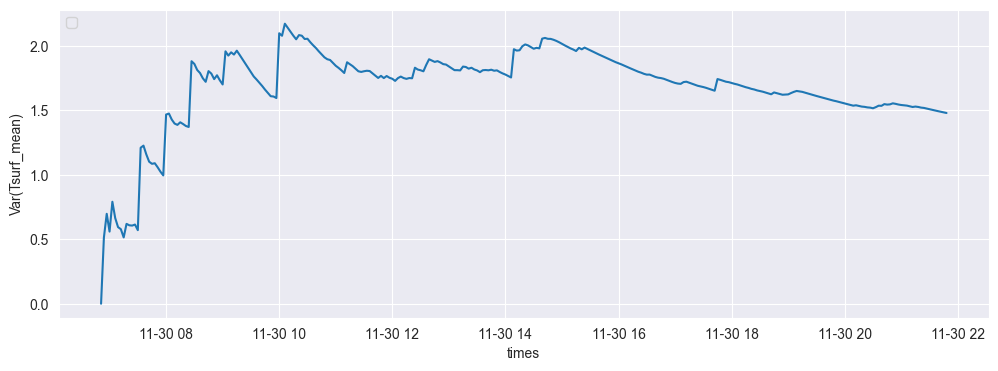
\includegraphics[width=\linewidth]{var3}
   \end{minipage}
   \begin{minipage}{.48\textwidth}
     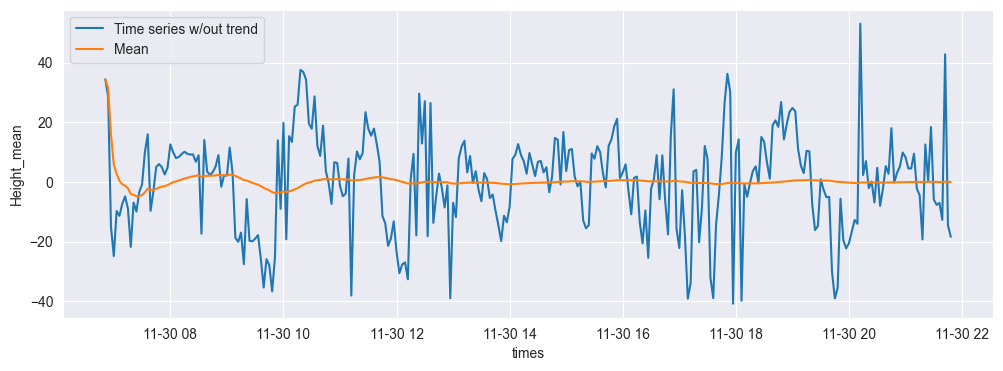
\includegraphics[width=\linewidth]{mean4}
   \end{minipage} \hfill
\begin{minipage}{.48\textwidth}
     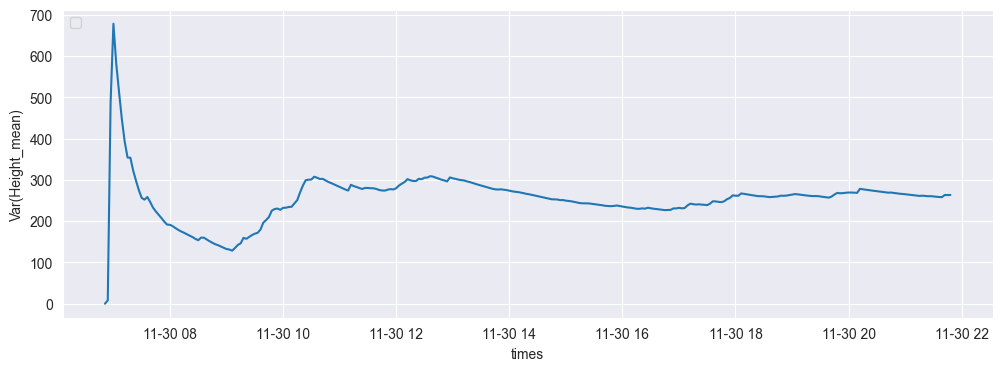
\includegraphics[width=\linewidth]{var4}
   \end{minipage}
   \begin{minipage}{.48\textwidth}
     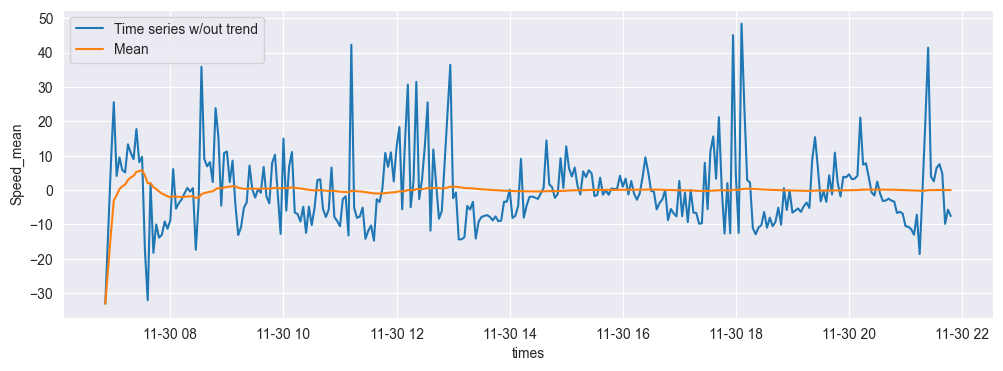
\includegraphics[width=\linewidth]{mean5}
   \end{minipage} \hfill
\begin{minipage}{.48\textwidth}
     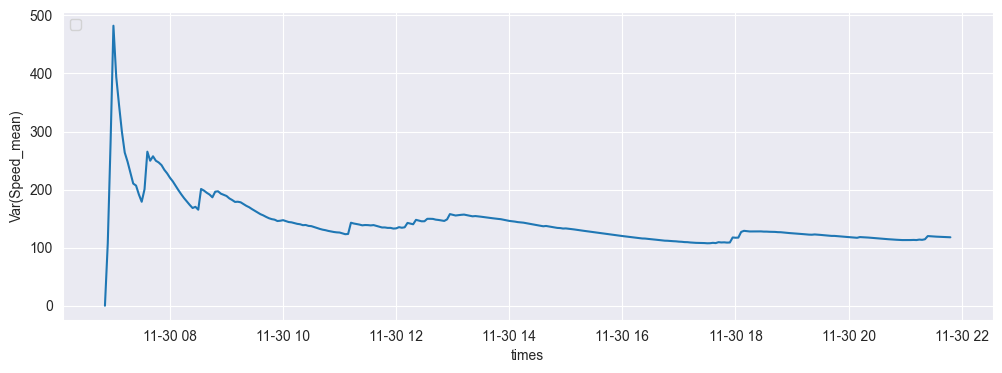
\includegraphics[width=\linewidth]{var5}
   \end{minipage}
\caption{The histogram of the generated sample vs the mixture's density and the histogram of observed Friction\_mean}
\label{fig: 2}
\end{figure}

One can observe that the estimates of mean functions looks constant for all of the modified series. As for the variance, as soon as it stabilizes, it fluctuates a bit near some horizontal line for all of the features. Also we analyzed autocovariance functions for the features which are presented in figure \ref{fig: 3}. All of them look approximately constant what also shows that the processes are stationary in the weak sense. To conclude the topic of stationarity, we did Augmented Dickey-Fuller (ADF) to finalize our conclusion.  

ADF test checks the hypothesis on whether the given time series is I(1) (i.e. the time series of its differences is stationary but it is not) versus I(0) alternative hypothesis assuming that its structure is described by an ARMA model white noise errors. The test estimates the regression coefficient $\phi$ and the regression:
\[ y_t = \mathbf{\beta}^T \mathbf{D}_t + \phi y_{t-1}  + \sum_{j=1}^{q} \psi_j \Delta y_{t-j} + \eps_t, \]
where $\beta$ is a vector of coefficients for components in $\mathbf{D}_t$ which determines deterministic part of the series, i.e. trend or seasonality, $\Delta y_\tau = y_{\tau} - y_{\tau-1}$. Given the OLS estimates $\widehat{\phi}$ and $\widehat{\psi}_k$ of the coefficients $\phi$ and $\psi_k$, the test statistic is
\[ t_{\text{ADF}} = T\frac{\widehat{\phi}-1}{1 - \sum_{j=1}^{q} \widehat{\psi}_j}, \]
where $T$ is the time series' time range. The test statistic distribution has its own tabulated distribution and limiting distribution under some assumptions. The parameter $q$ determines the lag length in the aforementioned regression. If it is too large, the test's power suffers. If it is too small, the test becomes biased \cite{Zivot01}.

\begin{figure}[!h]
   \begin{minipage}{.48\textwidth}
     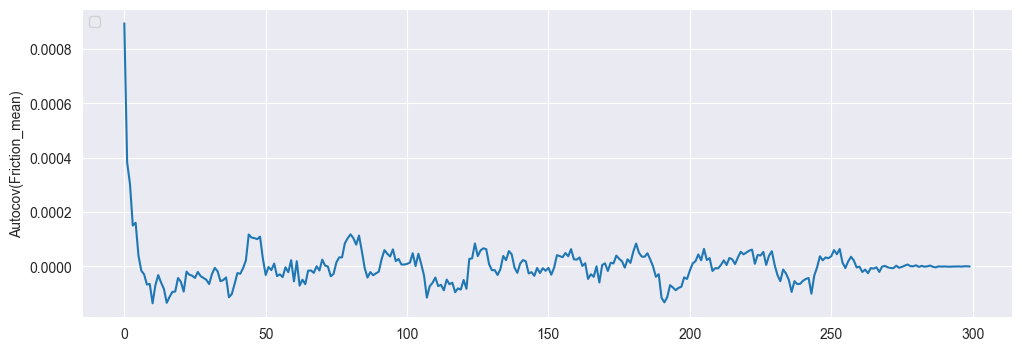
\includegraphics[width=\linewidth]{acov1}
   \end{minipage} \hfill
\begin{minipage}{.48\textwidth}
     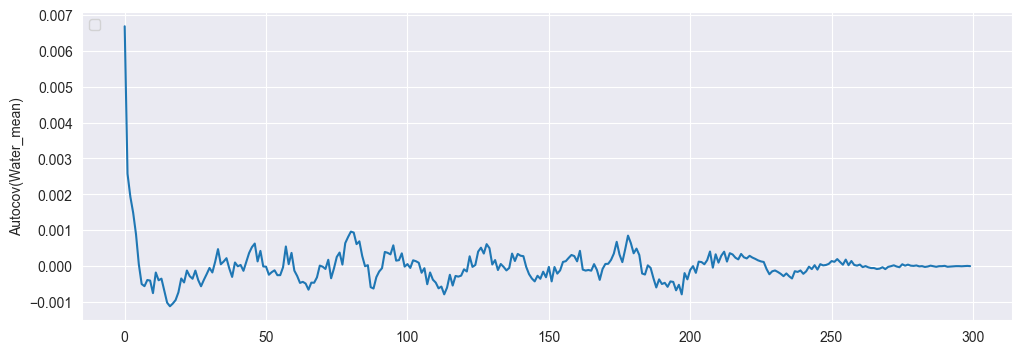
\includegraphics[width=\linewidth]{acov2}
   \end{minipage}\\
\begin{minipage}{.48\textwidth}
     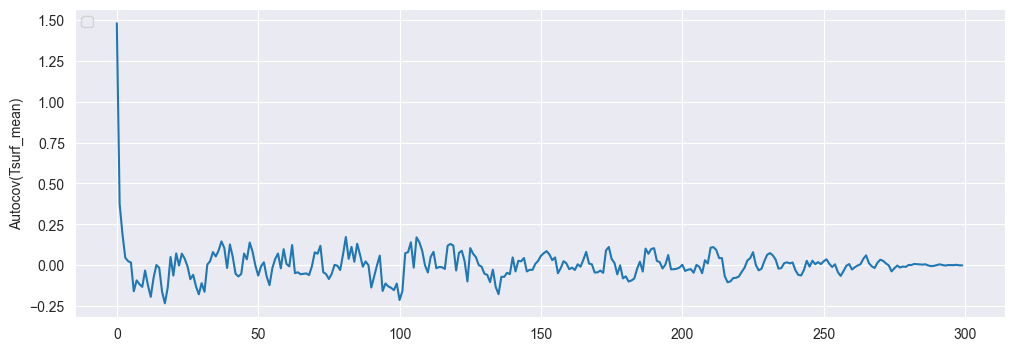
\includegraphics[width=\linewidth]{acov3}
   \end{minipage} \hfill
\begin{minipage}{.48\textwidth}
     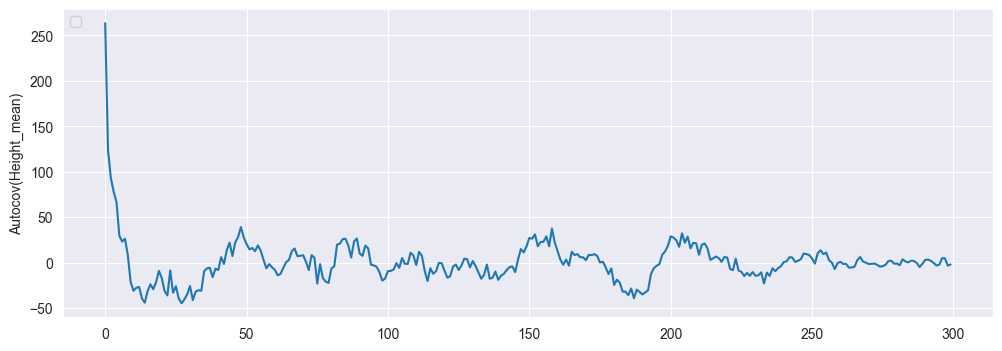
\includegraphics[width=\linewidth]{acov4}
   \end{minipage}\\
\centering
\begin{minipage}{.48\textwidth}
     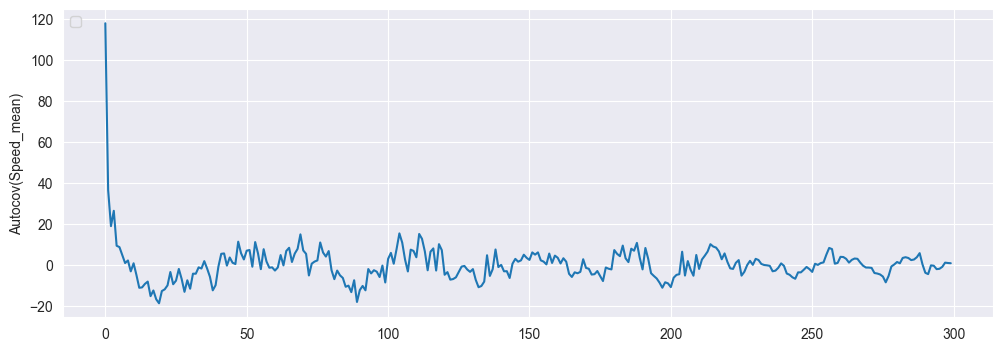
\includegraphics[width=\linewidth]{acov5}
   \end{minipage}
\caption{The histogram of the generated sample vs the mixture's density and the histogram of observed Friction\_mean}
\label{fig: 3}
\end{figure}

The results of the test for our time series are as follows:
\begin{outline}
\1 ADF test rejects the hypothesis on Friction\_mean having unit root, p-value $\approx 3.2\cdot 10^{-11}$ with $q = 1$;
\1 the same for Water\_mean, p-value $\approx 3.24\cdot 10^{-9}$ with $q = 5$;
\1 the same for Tsurf\_mean, p-value $\approx 5.8 \cdot 10^{-25}$ with $q = 0$;
\1 the same for Height\_mean, p-value $\approx 1.0\cdot 10^{-6}$ with $q = 4$;
\1 the same for Water\_mean, p-value $\approx 1.9\cdot 10^{-9}$ with $q = 1$.
\end{outline}

So we are allowed to treat the resulted time series as stationary ones.

\section{Cross-correlation function analysis}

We did the research of cross-correlation between our targets and predictors. Their plots are presented in figure \ref{fig: 4} and they show no strong linear connections between the variables.

\begin{figure}[!h]
   \begin{minipage}{.48\textwidth}
     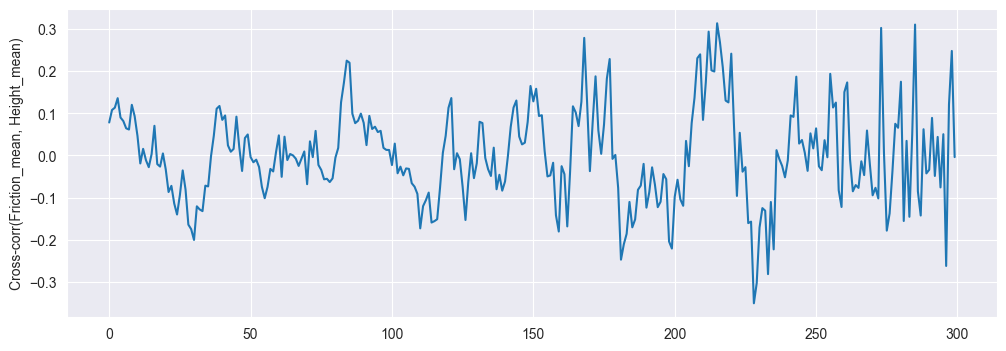
\includegraphics[width=\linewidth]{ccf1}
   \end{minipage} \hfill
\begin{minipage}{.48\textwidth}
     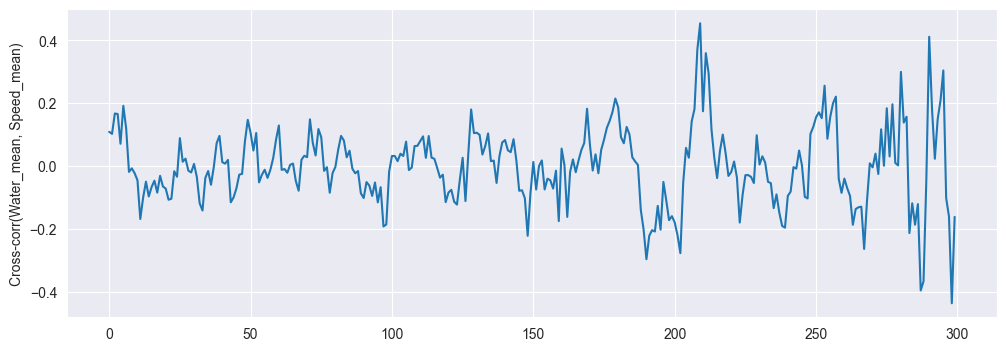
\includegraphics[width=\linewidth]{ccf4}
   \end{minipage}
   \begin{minipage}{.48\textwidth}
     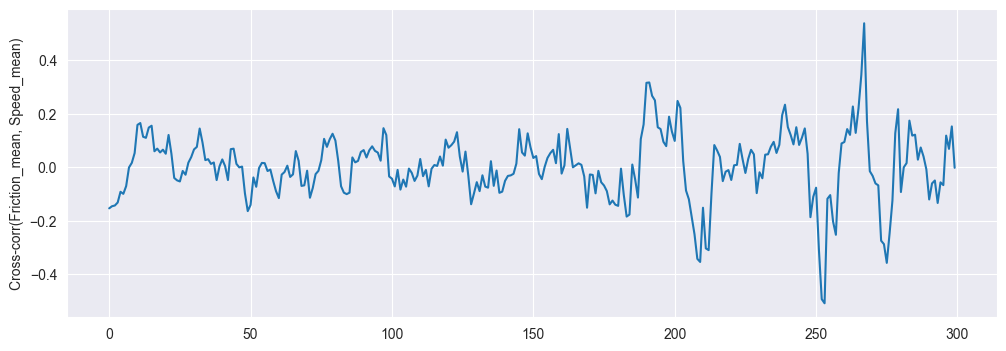
\includegraphics[width=\linewidth]{ccf2}
   \end{minipage} \hfill
\begin{minipage}{.48\textwidth}
     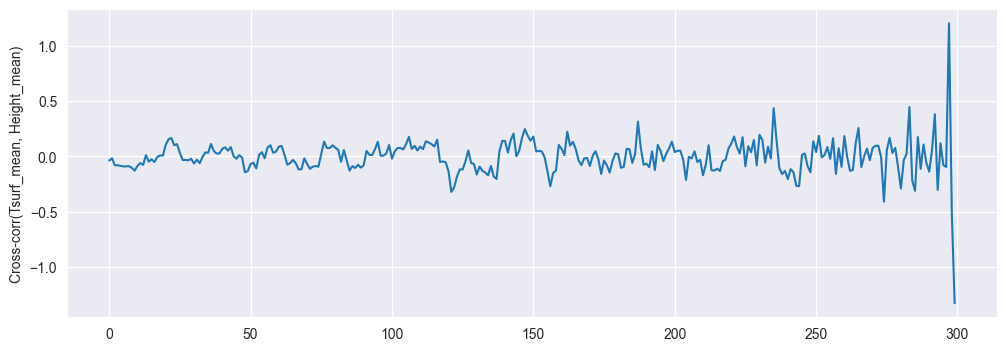
\includegraphics[width=\linewidth]{ccf5}
   \end{minipage}
   \begin{minipage}{.48\textwidth}
     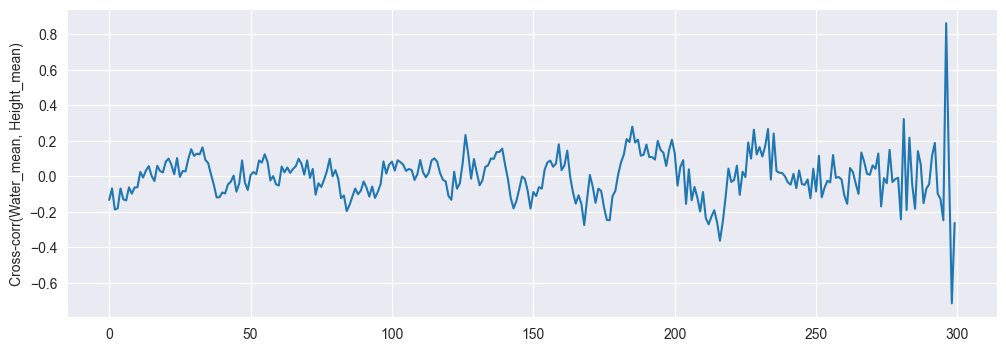
\includegraphics[width=\linewidth]{ccf3}
   \end{minipage} \hfill
\begin{minipage}{.48\textwidth}
     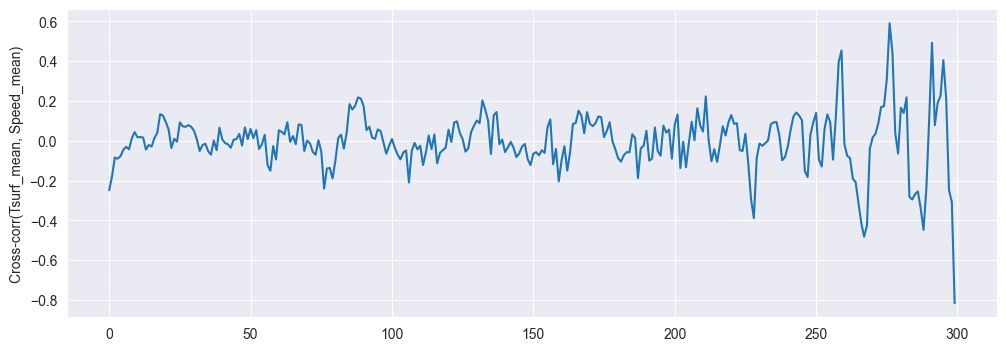
\includegraphics[width=\linewidth]{ccf6}
   \end{minipage}
\caption{The histogram of the generated sample vs the mixture's density and the histogram of observed Friction\_mean}
\label{fig: 4}
\end{figure}


\section{Noise filtration}
\section{Estimation of spectral density function}
\section{Auto-regression model}
\section{Model in a form of linear dynamical system}



\section{Appendix}
The Python notebook related to the aforementioned calculations is presented in Github \cite{repogithub}.

{\small \bibliography{biblio}}
\bibliographystyle{gost2008}

\end{document}